\normalsize
\subsection[pes\_samples]{pes\_samples.py}
This module provides two examples of potential energy surfaces for benchmarking purposes. Both inherits from
"problem.tem\-plate", thus having the corresponding \func{get\_*} methods. The \func{muller\_brown} corresponds
to the M\"uller-Brown potential, which presents a couple of minimums at [-0.558, 1.442] and [0.624, 0.028], 
and a transition state around [-0.822, 0.624].\\
The \func{cerjan\_miller} potential accounts for the Cerjan-Miller expression:
\begin{equation*}
f(x,y) = \left( a - b \cdot y \right) x^2 e^{-x^2} + y^2\cdot \frac{c}{2}
\end{equation*}
where a = 1.0, b = 1.2 and c = 1.0.
This surface presents three minima at [-2.9, 0.0], [0.0, 0.0] and [2.9, 0.0]; and two transition states at [-1.0, 0.1] and [1.0, 0.1].
\\
Both classes implements analytical gradient and hessian.
\begin{pyglist}[language=python,fvset={frame=single}]
class muller_brown()
    def get_func()
    def get_grad()
    def get_hess()

class cerjan_miller()
    def get_func()
    def get_grad()
    def get_hess()
\end{pyglist}
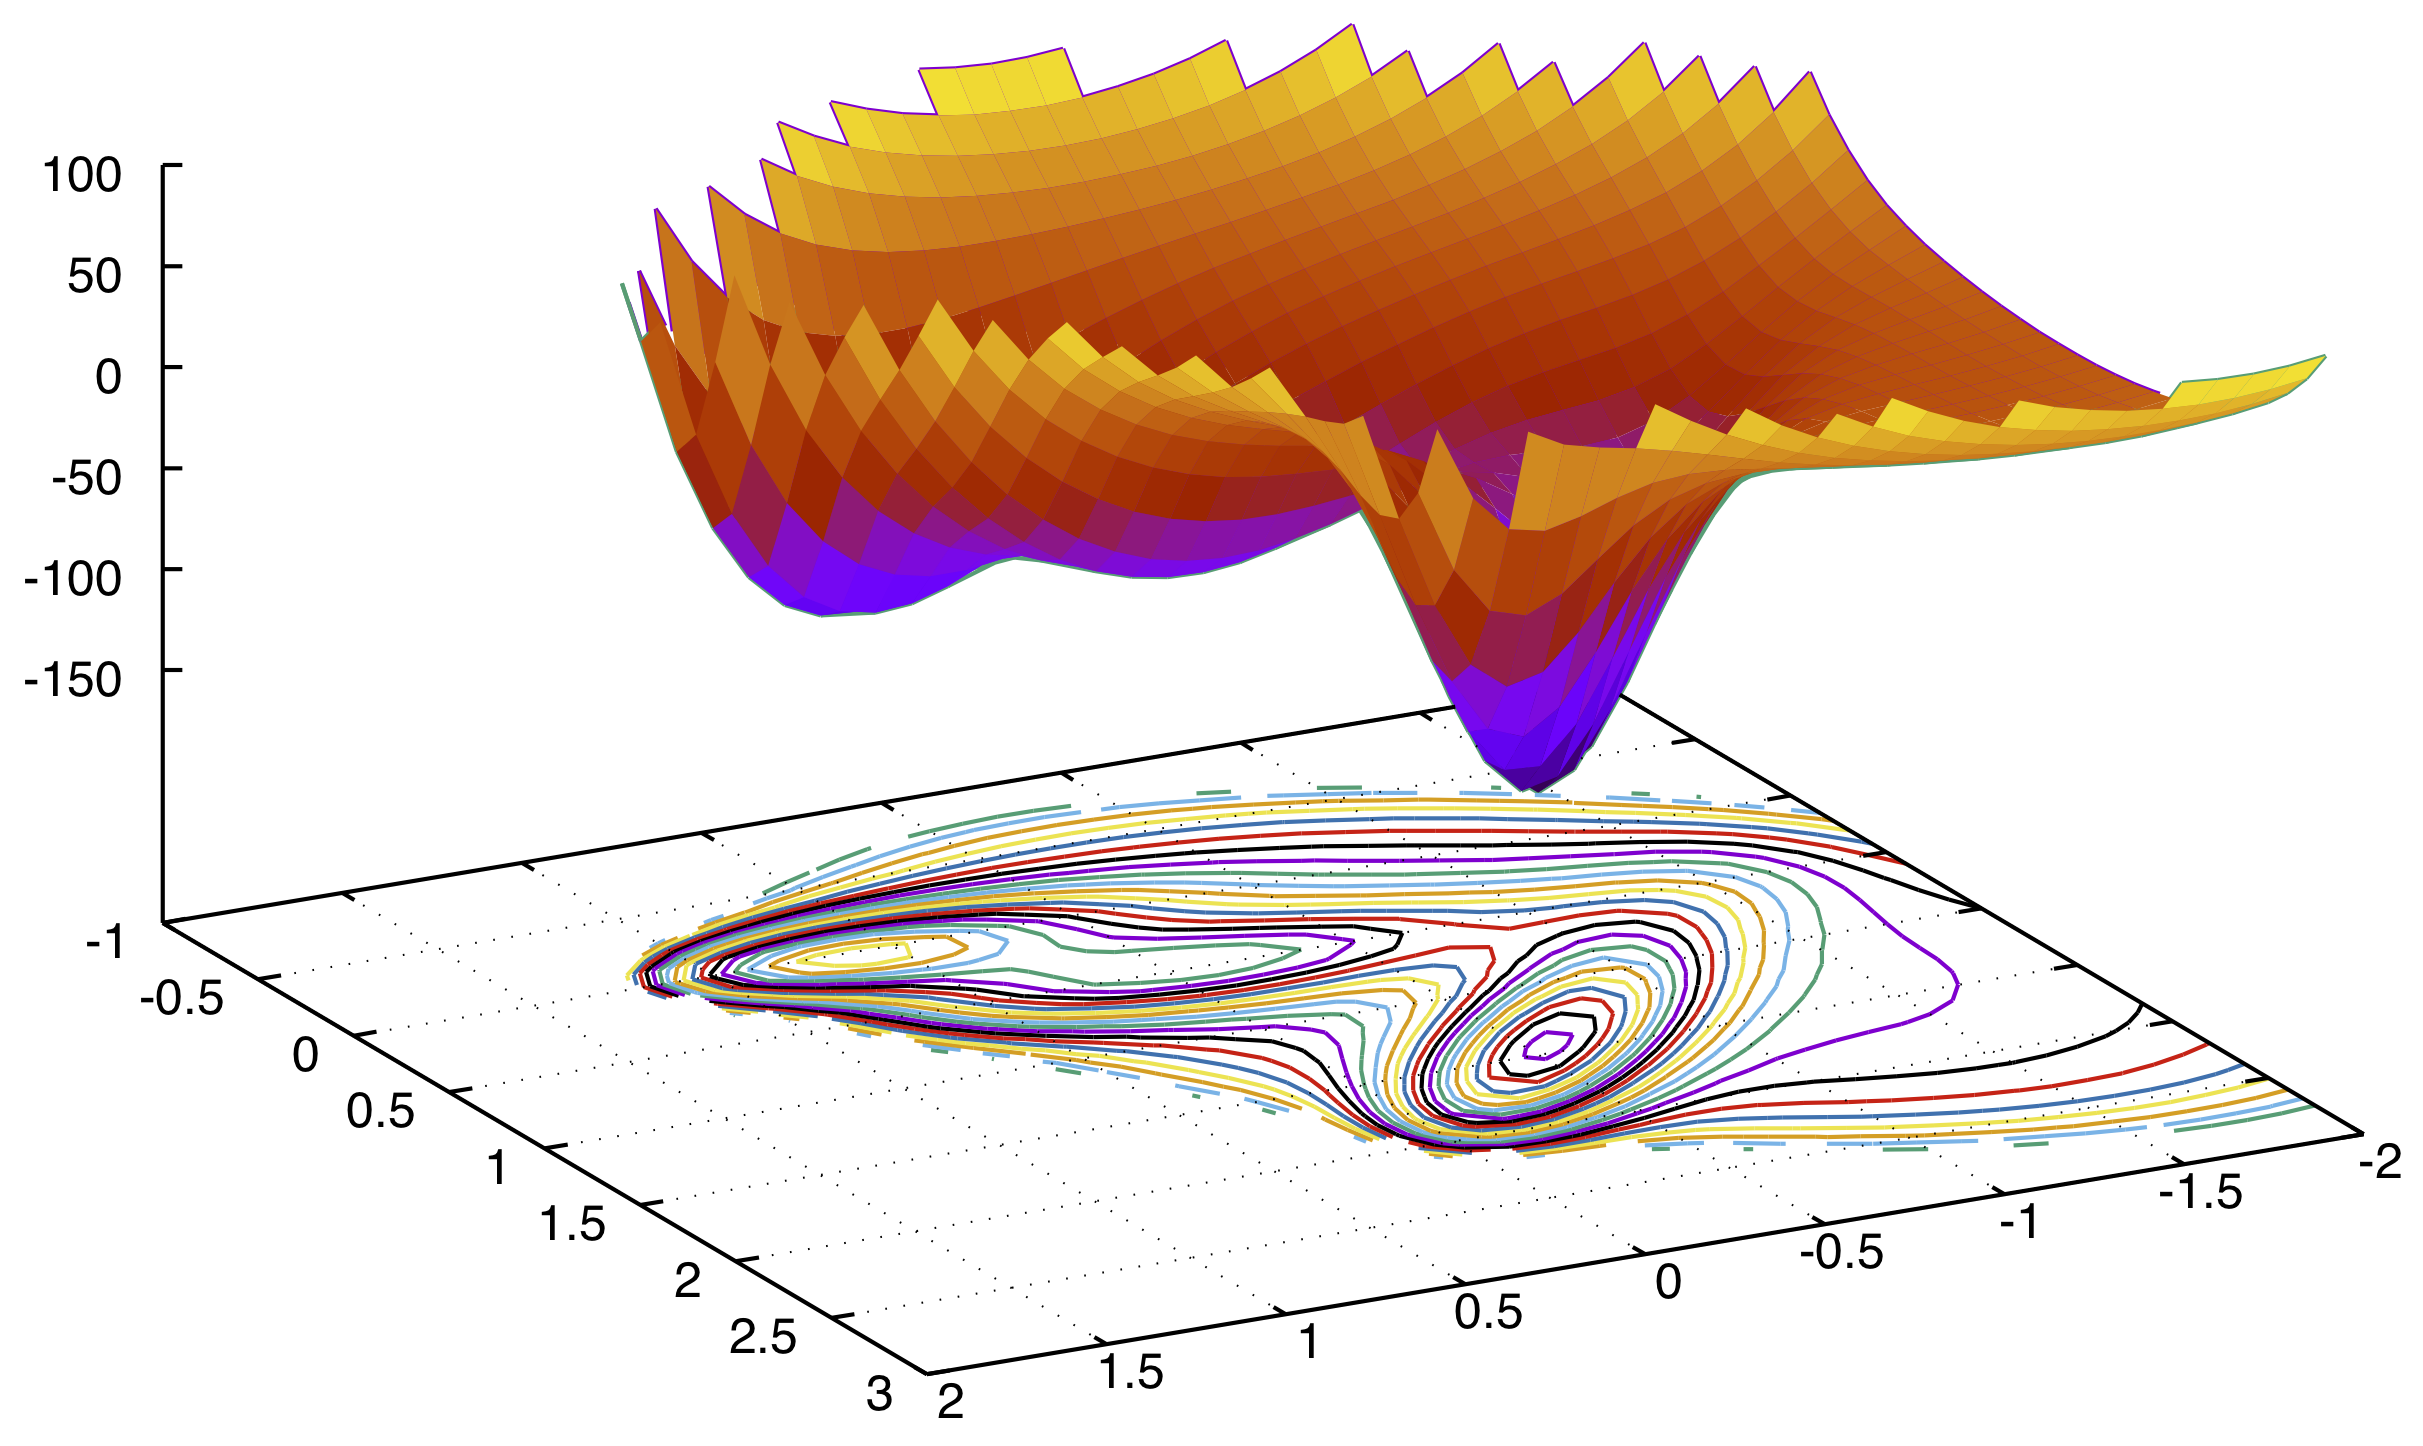
\includegraphics[width=.5\textwidth]{12.png}
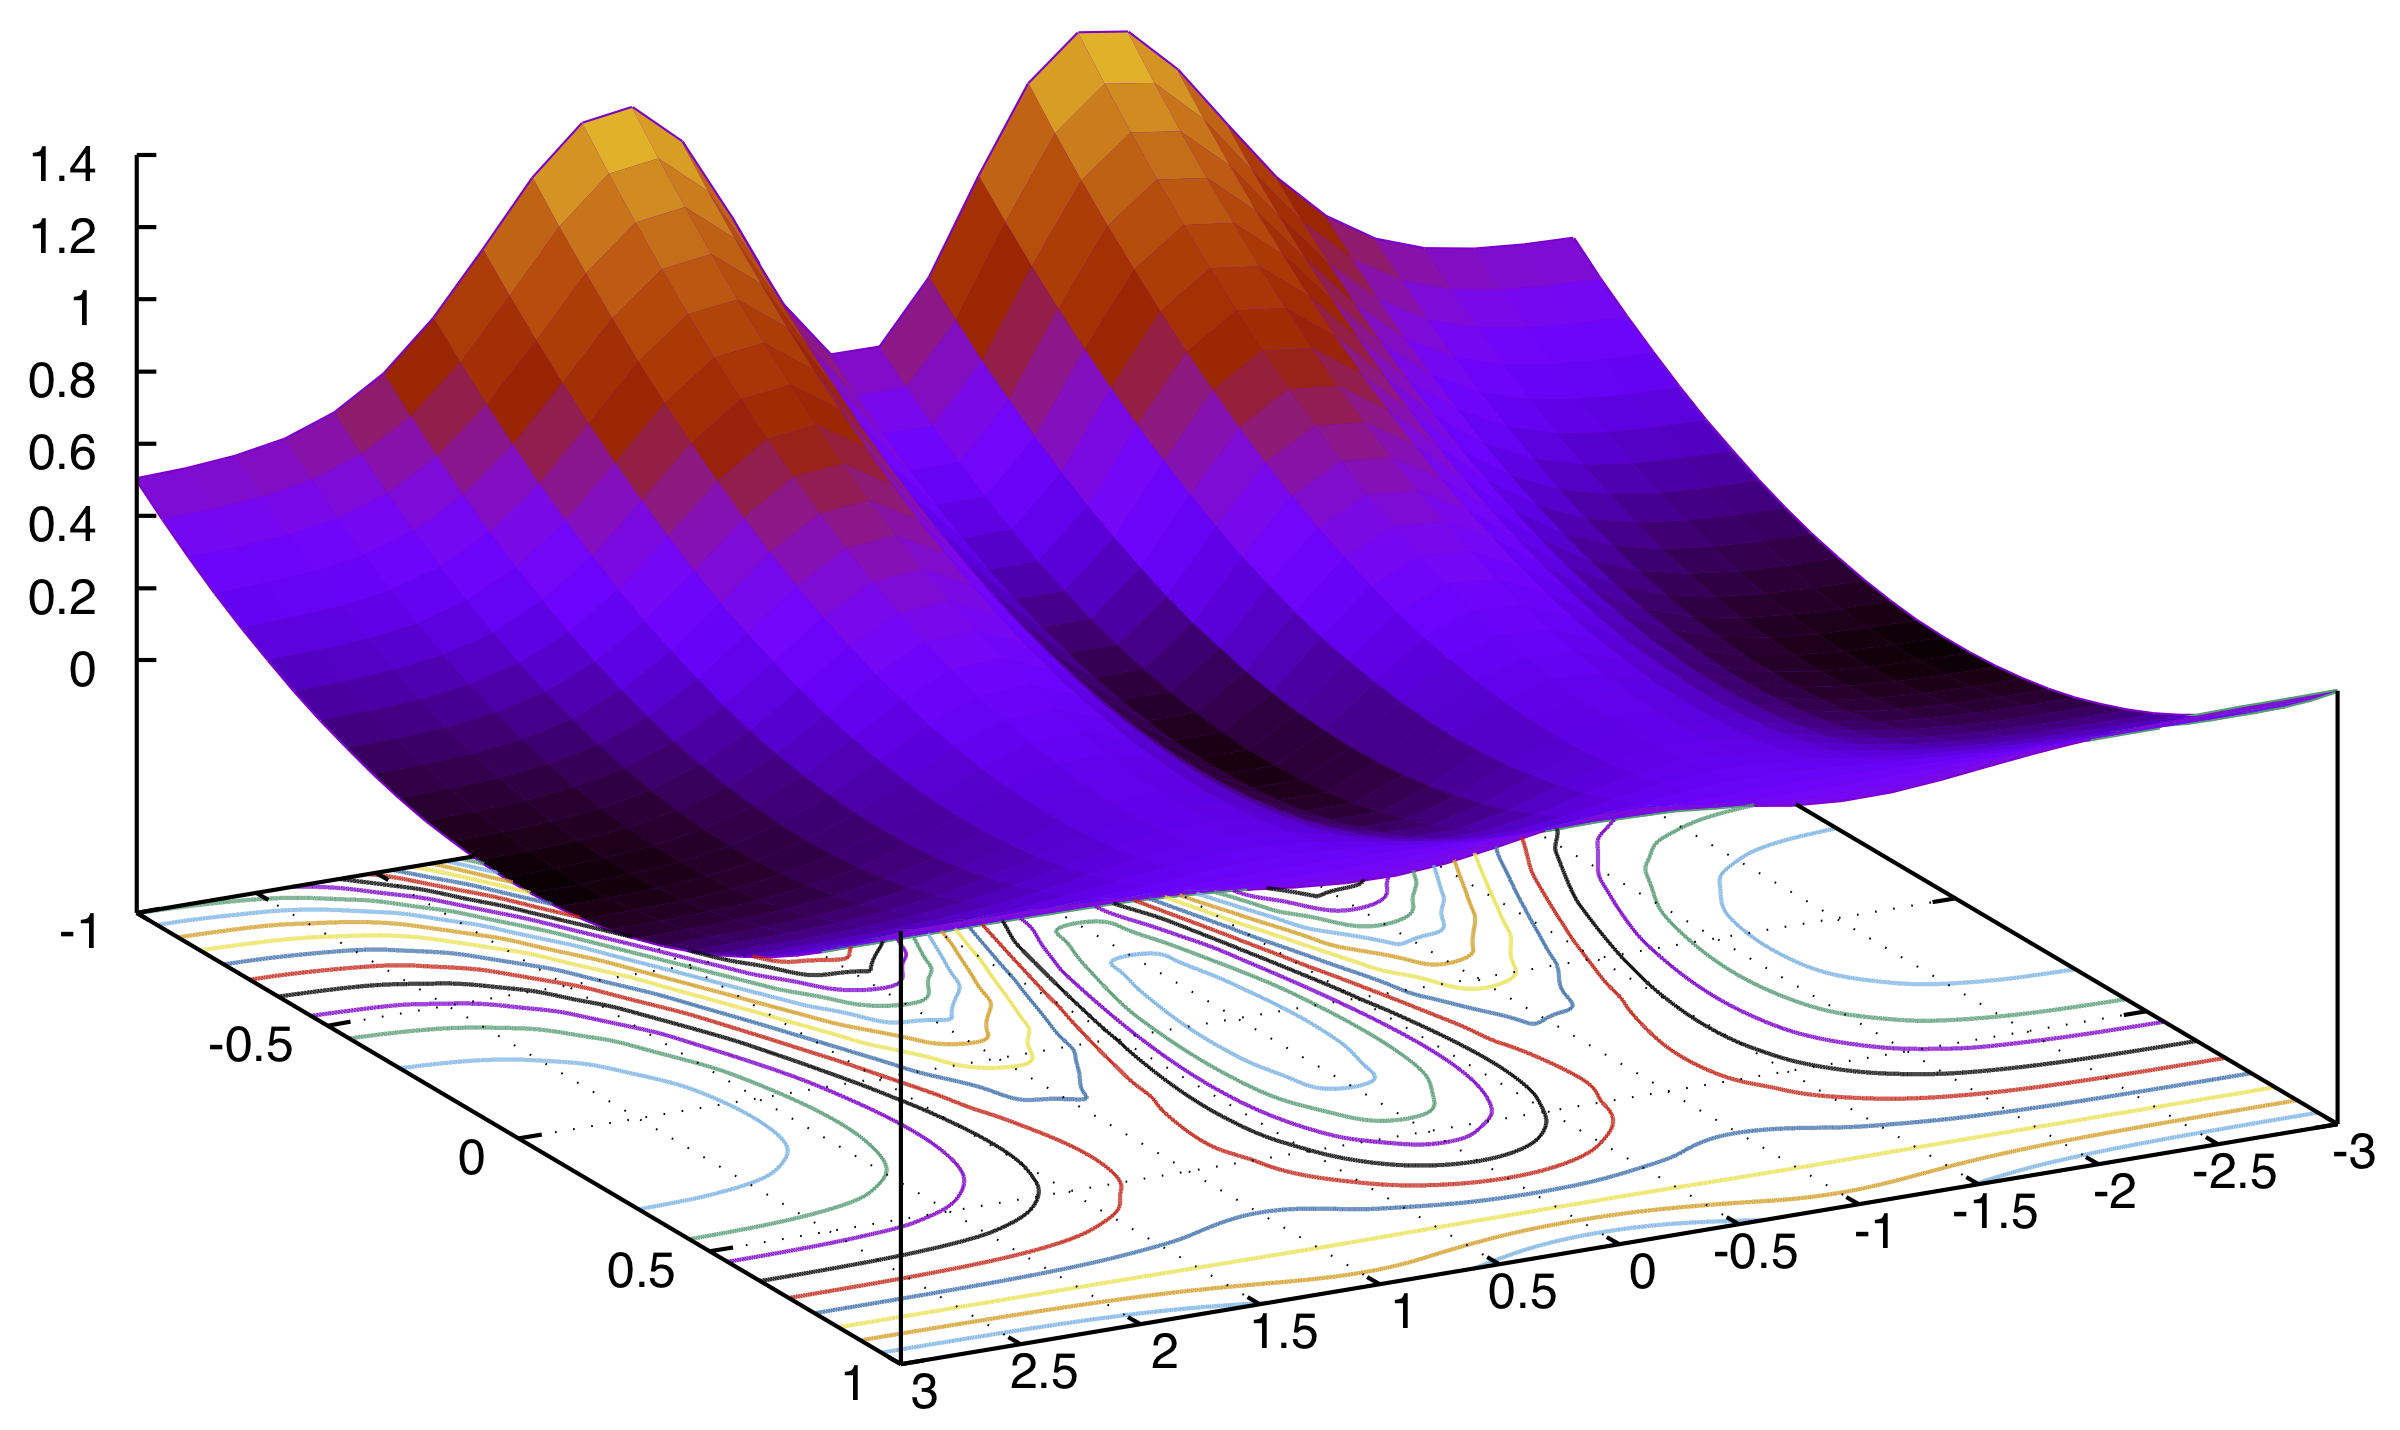
\includegraphics[width=.5\textwidth]{13.png}
%\footnotesize
%\begin{pyglist}[language=python,fvset={frame=single}]
%\end{pyglist}
